%=========================================================================
% fig-tut3-gcd-dpath
%=========================================================================

%\begin{figure}
  \centering

  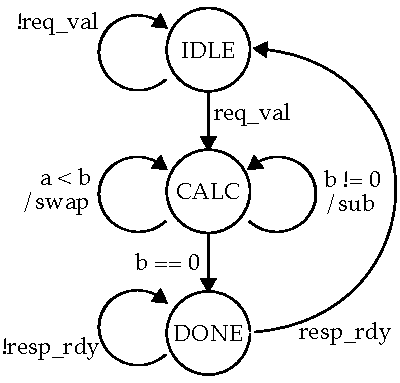
\includegraphics[width=\tw]{tut3-gcd-ctrl.svg.pdf}

  \caption{\textbf{FSM Diagram for GCD --} A hybrid Moore/Mealy FSM for
    controlling the datapath in Figure~\ref{fig-tut3-gcd-dpath}. Mealy
    transitions in the calc state determine whether to swap or subtract.}
  \label{fig-tut3-gcd-ctrl}

%\end{figure}

